
%% Impulse and Momentum Questions used on the
%% NYSED Physics Regents Examination
%%--------------------------------------------------

%% this section contains 58 problems


%% Section June2015
%%--------------------
\element{nysed}{
\begin{question}{June2015-Q10}
    A \SI{0.0600}{\kilo\gram} ball traveling at \SI{60.0}{\meter\per\second} hits a concrete wall. 
    What speed must a \SI{0.0100}{\kilo\gram} bullet have in order to hit the wall with the same magnitude of momentum as the ball?
    \begin{multicols}{2}
    \begin{choices}
        \wrongchoice{\SI{3.60}{\meter\per\second}}
        \wrongchoice{\SI{6.00}{\meter\per\second}}
      \correctchoice{\SI{360.}{\meter\per\second}}
        \wrongchoice{\SI{600.}{\meter\per\second}}
    \end{choices}
    \end{multicols}
\end{question}
}


%% Section June2014
%%--------------------
\element{nysed}{
\begin{question}{June2014-Q09}
    A \SI{3.0}{\kilo\gram} object is acted upon by an impulse having a magnitude of \SI{15}{\newton\second}.
    What is the magnitude of the object's change in momentum due to this impulse?
    \begin{multicols}{2}
    \begin{choices}
        %% NOTE: Newton seconds?
      \correctchoice{\SI{15}{\kilo\gram\meter\per\second}}
        \wrongchoice{\SI{5.0}{\kilo\gram\meter\per\second}}
        \wrongchoice{\SI{3.0}{\kilo\gram\meter\per\second}}
        \wrongchoice{\SI{45}{\kilo\gram\meter\per\second}}
    \end{choices}
    \end{multicols}
\end{question}
}

\element{nysed}{
\begin{question}{June2014-Q10}
    An air bag is used to safely decrease the momentum of a driver in a car accident.
    The air bag reduces the magnitude of the force acting on the driver by:
    \begin{choices}
      \correctchoice{increasing the length of time the force acts on the driver}
        \wrongchoice{decreasing the distance over which the force acts on the driver}
        \wrongchoice{increasing the rate of acceleration of the driver}
        \wrongchoice{decreasing the mass of the driver}
    \end{choices}
\end{question}
}

\element{nysed}{
\begin{question}{June2014-Q16}
    A \SI{15}{\kilo\gram} cart is at rest on a horizontal surface.
    A \SI{5}{\kilo\gram} box is placed in the cart.
    Compared to the mass and inertia of the cart,
        the cart-box system has:
    \begin{choices}
      \correctchoice{more mass and more inertia}
        \wrongchoice{more mass and the same inertia}
        \wrongchoice{the same mass and more inertia}
        \wrongchoice{less mass and more inertia}
    \end{choices}
\end{question}
}


%% Section June2013
%%--------------------
\element{nysed}{
\begin{question}{June2013-Q01}
    Which term identifies a scalar quantity?
    \begin{multicols}{2}
    \begin{choices}
        \wrongchoice{displacement}
        \wrongchoice{momentum}
        \wrongchoice{velocity}
      \correctchoice{time}
    \end{choices}
    \end{multicols}
\end{question}
}

\element{nysed}{
\begin{question}{June2013-Q07}
    Which object has the greatest inertia?
    \begin{choices}
        \wrongchoice{a \SI{0.010}{\kilo\gram} bullet traveling at \SI{90}{\meter\per\second}}
        \wrongchoice{a \SI{30}{\kilo\gram} child traveling at \SI{10}{\meter\per\second} on her bike}
        \wrongchoice{a \SI{490}{\kilo\gram} elephant walking with a speed of \SI{1.0}{\meter\per\second}}
      \correctchoice{a \SI{1500}{\kilo\gram} car at rest in a parking lot}
    \end{choices}
\end{question}
}

\element{nysed}{
\begin{question}{June2013-Q37}
    The diagram below shows an \SI{8.0}{\kilo\gram} cart moving to the right at \SI{4.0}{\meter\per\second} about to make a head-on collision with a \SI{4.0}{\kilo\gram} cart moving to the left at \SI{6.0}{\meter\per\second}.
    \begin{center}
    \begin{tikzpicture}
        %% Ground
        \node[anchor=north,fill,pattern=north east lines,minimum width=8cm, minimum height=0.05cm] at (0,0) {};
        \draw (-4,0) -- (4,0);
        %% left Cart
        \node[draw,minimum height=1.1cm,minimum width=1.7cm,anchor=south] (L) at (-2.5,0.2) {\SI{8.0}{\kilo\gram}};
        \draw[fill=white] (L.south west) ++(0:0.4) circle (0.2);
        \draw[fill=black] (L.south west) ++(0:0.4) circle (1pt);
        \draw[fill=white] (L.south east) ++(180:0.4) circle (0.2);
        \draw[fill=black] (L.south east) ++(180:0.4) circle (1pt);
        \draw[thick,->] (L.east) -- ++(0:1) node[pos=0,anchor=south west] {\SI{4.0}{\meter\per\second}};
        %% right Cart
        \node[draw,minimum height=0.8cm,minimum width=1.2cm,anchor=south] (R) at (+2.5,0.2) {\SI{4.0}{\kilo\gram}};
        \draw[fill=white] (R.south west) ++(0:0.3) circle (0.2);
        \draw[fill=black] (R.south west) ++(0:0.3) circle (1pt);
        \draw[fill=white] (R.south east) ++(180:0.3) circle (0.2);
        \draw[fill=black] (R.south east) ++(180:0.3) circle (1pt);
        \draw[thick,->] (R.west) -- ++(180:1.5) node[pos=0.5,anchor=south] {\SI{6.0}{\meter\per\second}};
    \end{tikzpicture}
    \end{center}
    After the collision, the \SI{4.0}{\kilo\gram} cart moves to the right at \SI{3.0}{\meter\per\second}.
    What is the velocity of the \SI{8.0}{\kilo\gram} cart after the collision?
    \begin{multicols}{2}
    \begin{choices}
      \correctchoice{\SI{0.50}{\meter\per\second} left}
        \wrongchoice{\SI{0.50}{\meter\per\second} right}
        \wrongchoice{\SI{5.5}{\meter\per\second} left}
        \wrongchoice{\SI{5.5}{\meter\per\second} right}
    \end{choices}
    \end{multicols}
\end{question}
}


%% Section June2012
%%--------------------
\element{nysed}{
\begin{question}{June2012-Q05}
    Which object has the greatest inertia?
    \begin{choices}
      \correctchoice{a \SI{15}{\kilo\gram} mass traveling at \SI{5.0}{\meter\per\second}}
        \wrongchoice{a \SI{10}{\kilo\gram} mass traveling at \SI{10}{\meter\per\second}}
        \wrongchoice{a \SI{10}{\kilo\gram} mass traveling at \SI{5.0}{\meter\per\second}}
        \wrongchoice{a \SI{5.0}{\kilo\gram} mass traveling at \SI{15}{\meter\per\second}}
    \end{choices}
\end{question}
}

\element{nysed}{
\begin{question}{June2012-Q10}
    A \SI{5.00}{\kilo\gram} block slides along a horizontal frictionless surface at \SI{10.0}{\meter\per\second} for \SI{4.00}{\second}.
    The magnitude of the block's momentum is:
    \begin{multicols}{2}
    \begin{choices}
        \wrongchoice{\SI{200}{\kilo\gram\meter\per\second}}
      \correctchoice{\SI{50.0}{\kilo\gram\meter\per\second}}
        \wrongchoice{\SI{20.0}{\kilo\gram\meter\per\second}}
        \wrongchoice{\SI{12.5}{\kilo\gram\meter\per\second}}
    \end{choices}
    \end{multicols}
\end{question}
}

\element{nysed}{
\begin{question}{June2012-Q38}
    When a \SI{1.0}{\kilo\gram} cart moving with a speed of \SI{0.50}{\meter\per\second} on a horizontal surface collides with a second \SI{1.0}{\kilo\gram} cart initially at rest, the carts lock together.
    What is the speed of the combined carts after the collision?
    [Neglect friction.]
    \begin{multicols}{2}
    \begin{choices}
        \wrongchoice{\SI{1.0}{\meter\per\second}}
        \wrongchoice{\SI{0.50}{\meter\per\second}}
      \correctchoice{\SI{0.25}{\meter\per\second}}
        \wrongchoice{\SI{0}{\meter\per\second}}
    \end{choices}
    \end{multicols}
\end{question}
}


%% Section June2011
%%--------------------
\element{nysed}{
\begin{question}{June2011-Q13}
    As shown in the diagram below,
        an open box and its contents have a combined mass of \SI{5.0}{\kilo\gram}.
    A horizontal force of \SI{15}{\newton} is required to push the box at a constant speed of \SI{1.5}{\meter\per\second} across a level surface.
    \begin{center}
    \begin{tikzpicture}
        %% Ground
        \node[anchor=north,fill,pattern=north east lines,minimum width=8cm, minimum height=0.05cm] at (0,0) {};
        \draw (-4,0) -- (4,0);
        \node[anchor=north,yshift=-1em] at (0,0) {level surface};
        %% box
        \node[draw,anchor=south,minimum size=2cm] (A) at (0,0) {\SI{5.0}{\kilo\gram}};
        \node[anchor=south] at (A.north) {Box};
        \draw[thick,<-] (A.west) -- ++(180:2) node[pos=0.5,anchor=south] {$F=\SI{15}{\newton}$};
        \draw[thick,->] (A.north east) ++ (0.1,0.1) -- ++(0:2) node[pos=0.5,anchor=south] {$v=\SI{1.5}{\meter\per\second}$};
    \end{tikzpicture}
    \end{center}
    The inertia of the box and its contents increases if there is an increase in the:
    \begin{choices}
        \wrongchoice{speed of the box}
      \correctchoice{mass of the contents of the box}
        \wrongchoice{magnitude of the horizontal force applied to the box}
        \wrongchoice{coefficient of kinetic friction between the box and the level surface}
    \end{choices}
\end{question}
}


%% Section June2010
%%--------------------
\element{nysed}{
\begin{question}{June2010-Q09}
    The data table below lists the mass and speed of four different objects.
    Which object has the greatest inertia?
    \begin{center}
    \begin{tabu}{cX[c]X[c]}
        \toprule
        \makebox[1.5em][c]{\textnumero}
        & Mass/(\si{\kilo\gram}) & Speed/(\si{\meter\per\second}) \\
        \bottomrule
    \end{tabu}
    \end{center}
    \begin{choices}
        \wrongchoice{\begin{tabu}{X[c]X[c]}   4.0 & 6.0 \\ \end{tabu}}
        \wrongchoice{\begin{tabu}{X[c]X[c]}   6.0 & 5.0 \\ \end{tabu}}
        \wrongchoice{\begin{tabu}{X[c]X[c]}   8.0 & 3.0 \\ \end{tabu}}
      \correctchoice{\begin{tabu}{X[c]X[c]}  16.0 & 1.5 \\ \end{tabu}}
    \end{choices}
\end{question}
}

\element{nysed}{
\begin{question}{June2010-Q13}
    A \SI{3.1}{\kilo\gram} gun initially at rest is free to move.
    When a \SI{0.015}{\kilo\gram} bullet leaves the gun with a speed of \SI{500}{\meter\per\second},
        what is the speed of the gun?
    \begin{multicols}{2}
    \begin{choices}
        \wrongchoice{\SI{0.0}{\meter\per\second}}
      \correctchoice{\SI{2.4}{\meter\per\second}}
        \wrongchoice{\SI{7.5}{\meter\per\second}}
        \wrongchoice{\SI{500}{\meter\per\second}}
    \end{choices}
    \end{multicols}
\end{question}
}


%% Section June2009
%%--------------------
\element{nysed}{
\begin{question}{June2009-Q03}
    Which quantity is a vector?
    \begin{multicols}{2}
    \begin{choices}
      \correctchoice{impulse}
        \wrongchoice{power}
        \wrongchoice{speed}
        \wrongchoice{time}
    \end{choices}
    \end{multicols}
\end{question}
}


%% Section Jan2009
%%--------------------
\element{nysed}{
\begin{question}{Jan2009-Q06}
    Which object has the greatest inertia?
    \begin{choices}
        \wrongchoice{a falling leaf}
        \wrongchoice{a softball in flight}
      \correctchoice{a seated high school student}
        \wrongchoice{a rising helium-filled toy balloon}
    \end{choices}
\end{question}
}


%% Section June2008
%%--------------------
\element{nysed}{
\begin{question}{June2008-Q03}
    Cart $A$ has a mass of \SI{2}{\kilo\gram} and a speed of \SI{3}{\meter\per\second}.
    Cart $B$ has a mass of \SI{3}{\kilo\gram} and a speed of \SI{2}{\meter\per\second}.
    Compared to the inertia and magnitude of momentum of cart $A$, cart $B$ has:
    \begin{choices}
        \wrongchoice{the same inertia and a smaller magnitude of momentum}
        \wrongchoice{the same inertia and the same magnitude of momentum}
        \wrongchoice{greater inertia and a smaller magnitude of momentum}
      \correctchoice{greater inertia and the same magnitude of momentum}
    \end{choices}
\end{question}
}

\element{nysed}{
\begin{question}{June2008-Q14}
    A \SI{0.45}{\kilo\gram} football traveling at a speed of \SI{22}{\meter\per\second} is caught by an \SI{84}{\kilo\gram} stationary receiver.
    If the football comes to rest in the receiver's arms,
        the magnitude of the impulse imparted to the receiver by the ball is:
    \begin{multicols}{2}
    \begin{choices}
        \wrongchoice{\SI{1800}{\newton\second}}
      \correctchoice{\SI{9.9}{\newton\second}}
        \wrongchoice{\SI{4.4}{\newton\second}}
        \wrongchoice{\SI{3.8}{\newton\second}}
    \end{choices}
    \end{multicols}
\end{question}
}

\element{nysed}{
\begin{question}{June2008-Q43}
    The diagram below represents two masses before and after they collide.
    Before the collision, mass $m_A$ is moving to the right with speed $v$,
        and mass $m_B$ is at rest.
    Upon collision the two masses stick together.
    \begin{center}
        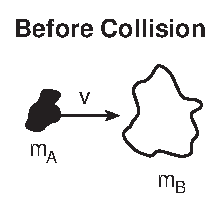
\includegraphics[keepaspectratio,scale=0.75]{June2008-Q43-left}
        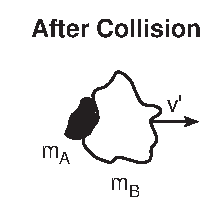
\includegraphics[keepaspectratio,scale=0.75]{June2008-Q43-right}
    \end{center}
    Which expression represents the speed, $v'$, of the masses after collision?
    Assume no outside forces are acting on $m_A$ or $m_B$.
    \begin{multicols}{2}
    \begin{choices}
        \wrongchoice{$\dfrac{m_A + m_B}{v}$}
        \wrongchoice{$\dfrac{m_A + m_B}{m_A v}$}
        \wrongchoice{$\dfrac{m_B v}{m_A + m_B}$}
      \correctchoice{$\dfrac{m_A v}{m_a + m_B}$}
    \end{choices}
    \end{multicols}
\end{question}
}


%% Section Jan2008
%%--------------------
\element{nysed}{
\begin{question}{Jan2008-Q05}
    Which object has the greatest inertia?
    \begin{choices}
        \wrongchoice{a \SI{5.00}{\kilo\gram} mass moving at \SI{10.0}{\meter\per\second}}
        \wrongchoice{a \SI{10.0}{\kilo\gram} mass moving at \SI{1.00}{\meter\per\second}}
        \wrongchoice{a \SI{15.0}{\kilo\gram} mass moving at \SI{10.0}{\meter\per\second}}
      \correctchoice{a \SI{20.0}{\kilo\gram} mass moving at \SI{1.00}{\meter\per\second}}
    \end{choices}
\end{question}
}

\element{nysed}{
\begin{question}{Jan2008-Q11}
    A \SI{6.0}{\kilo\gram} block, sliding to the east across a horizontal,
        frictionless surface with a momentum of \SI{30}{\kilo\gram\meter\per\second}, strikes an obstacle.
    The obstacle exerts an impulse of \SI{10}{\newton\second} to the west on the block.
    The speed of the block after the collision is:
    \begin{multicols}{2}
    \begin{choices}
        \wrongchoice{\SI{1.7}{\meter\per\second}}
      \correctchoice{\SI{3.3}{\meter\per\second}}
        \wrongchoice{\SI{5.0}{\meter\per\second}}
        \wrongchoice{\SI{20}{\meter\per\second}}
    \end{choices}
    \end{multicols}
\end{question}
}

\element{nysed}{
\begin{question}{Jan2008-Q13}
    A \SI{1.0}{\kilo\gram} laboratory car moving with a velocity of \SI{0.5}{\meter\per\second} due east collides with and sticks to a similar cart initially at rest.
    After the collision, the two carts move off together with a velocity of \SI{0.25}{\meter\per\second} due east.
    The total momentum of this frictionless system is:
    \begin{choices}
        \wrongchoice{zero before the collision}
        \wrongchoice{zero after the collision}
      \correctchoice{the same before and after the collision}
        \wrongchoice{greater before the collision than after the collision}
    \end{choices}
\end{question}
}


%% Section June2007
%%--------------------
\element{nysed}{
\begin{question}{June2007-Q09}
    Which situation will produce the greatest change of momentum for a \SI{1.0}{\kilo\gram} cart?
    \begin{choices}
      \correctchoice{applying a net force of \SI{5.0}{\newton} for \SI{2.0}{\second}}
        \wrongchoice{accelerating it from rest to \SI{3.0}{\meter\per\second}}
        \wrongchoice{accelerating it from \SI{2.0}{\meter\per\second} to \SI{4.0}{\meter\per\second}}
        \wrongchoice{applying a net force of \SI{10.0}{\newton} for \SI{0.5}{\second}}
    \end{choices}
\end{question}
}

\element{nysed}{
\begin{question}{June2007-Q42}
    In the diagram below, scaled vectors represent the momentum of each of two masses,
        $A$ and $B$, sliding toward each other on a frictionless, horizontal surface.
    \begin{center}
    %% NOTE: TODO: draw tikz
    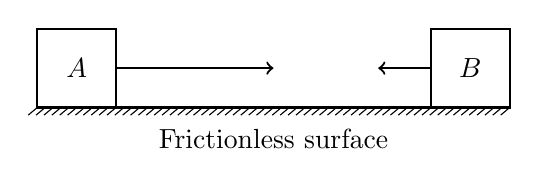
\begin{tikzpicture}
        %% Block A 2cm
        \draw[thick] (-3,0) rectangle (-2,1);
        \node[anchor=center] at (-2.5,0.5) {$A$};
        \draw[thick,->] (-2,0.5) -- (0.0,0.5);
        %% Block B 0.66cm
        \draw[thick] (3,0) rectangle (2,1);
        \node[anchor=center] at (2.5,0.5) {$B$};
        \draw[thick,->] (2,0.5) -- (1.33,0.5);
        %% Floor
        \draw[thick] (-3,0) -- (3,0);
        \foreach \x in {-30,-29,...,30}
            \draw[thin] (\x mm,0cm) -- ++ (220:0.15cm);
        \node[anchor=north] at (0,-0.15) {Frictionless surface};
    \end{tikzpicture}
    \end{center}
    What scaled vector best represents the momentum of the system after the masses collide?
    [Vectors are drawn to scale]
    \begin{multicols}{2}
    \begin{choices}
        \AMCboxDimensions{down=-0.25cm}
        \correctchoice{
            \begin{tikzpicture}
                \draw[white] (-0.5,-0.5) rectangle (2,0.5);
                \draw[thick,->] (0,0) -- (1.33,0);
            \end{tikzpicture}
        }
        \wrongchoice{
            \begin{tikzpicture}
                \draw[white] (-0.5,-0.5) rectangle (2,0.5);
                \draw[thick,->] (0,0) -- (2,0);
            \end{tikzpicture}
        }
        \wrongchoice{
            \begin{tikzpicture}
                \draw[white] (-0.5,-0.5) rectangle (2,0.5);
                \draw[thick,<-] (0,0) -- (0.66,0);
            \end{tikzpicture}
        }
        \wrongchoice{
            \begin{tikzpicture}
                \draw[white] (-0.5,-0.5) rectangle (2,0.5);
                \draw[thick,<-] (0,0) -- (1.33,0);
            \end{tikzpicture}
        }
    \end{choices}
    \end{multicols}
\end{question}
}


%% Section Jan2007
%%--------------------
\element{nysed}{
\begin{question}{Jan2007-Q08}
    A woman with horizontal velocity $v_1$ jumps off a dock into a stationary boat.
    After landing in the boat,
        the woman and the boat move with velocity $v_2$.
    Compared to velocity $v_1$, velocity $v_2$ has:
    \begin{choices}
      \correctchoice{smaller magnitude and the same direction}
        \wrongchoice{larger magnitude and the same direction}
        \wrongchoice{the same magnitude and the same direction}
        \wrongchoice{the same magnitude and opposite direction}
    \end{choices}
\end{question}
}

\element{nysed}{
\begin{question}{Jan2007-Q09}
    Which object has the greatest inertia?
    \begin{choices}
        \wrongchoice{a \SI{5.0}{\kilo\gram} object moving at a speed of \SI{5.0}{\meter\per\second}}
        \wrongchoice{a \SI{10}{\kilo\gram} object moving at a speed of \SI{3.0}{\meter\per\second}}
        \wrongchoice{a \SI{15}{\kilo\gram} object moving at a speed of \SI{1.0}{\meter\per\second}}
      \correctchoice{a \SI{20}{\kilo\gram} object at rest}
    \end{choices}
\end{question}
}


%% Section June2006
%%--------------------
\element{nysed}{
\begin{question}{June2006-Q05}
    Which object has the greatest inertia?
    \begin{choices}
        \wrongchoice{a \SI{1.0}{\kilo\gram} object moving at \SI{15}{\meter\per\second}}
        \wrongchoice{a \SI{5.0}{\kilo\gram} object at rest}
        \wrongchoice{a \SI{10}{\kilo\gram} object moving at \SI{2.0}{\meter\per\second}}
      \correctchoice{a \SI{15}{\kilo\gram} object at rest}
    \end{choices}
\end{question}
}

\element{nysed}{
\begin{question}{June2006-Q40}
    A \SI{3.0}{\kilo\gram} steel block is at rest on a friction-less horizontal surface.
    A \SI{1.0}{\kilo\gram} lump of clay is propelled horizontally at \SI{6.0}{\meter\per\second} toward the block as shown in the diagram below.
    \begin{center}
        %% NOTE: TODO: priority for tikz
        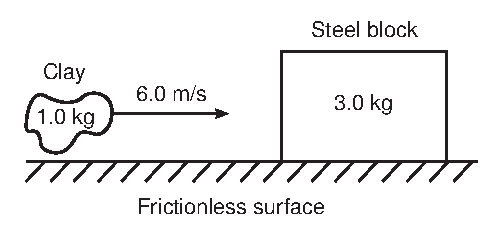
\includegraphics[keepaspectratio,scale=0.8]{June2006-Q40}
    \end{center}
    Upon collision,
        the clay and steel block stick together and move to the right with a speed of:
    \begin{multicols}{2}
    \begin{choices}
      \correctchoice{\SI{1.5}{\meter\per\second}}
        \wrongchoice{\SI{2.0}{\meter\per\second}}
        \wrongchoice{\SI{3.0}{\meter\per\second}}
        \wrongchoice{\SI{6.0}{\meter\per\second}}
    \end{choices}
    \end{multicols}
\end{question}
}


%% Section Jan2006
%%--------------------
\element{nysed}{
\begin{question}{Jan2006-Q45}
    In the diagram below, a block of mass $M$ initially at rest on a frictionless horizontal surface is struck by a bullet of mass $m$ moving with horizontal velocity $v$.
    \begin{center}
        %% NOTE: tikz would be easy
        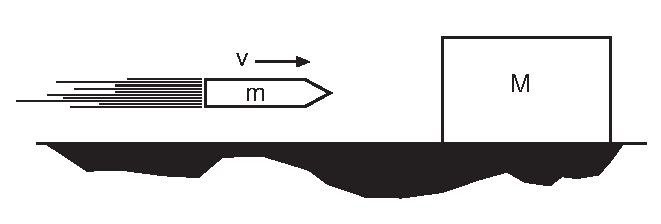
\includegraphics[keepaspectratio,scale=0.75]{Jan2006-Q45}
    \end{center}
    What is the velocity of the bullet-block system after the bullet embeds itself into the block?
    \begin{multicols}{2}
    \begin{choices}
        \wrongchoice{$\dfrac{M+v}{M}m$}
        \wrongchoice{$\dfrac{m+M}{m}v$}
        \wrongchoice{$\dfrac{m+v}{M}m$}
      \correctchoice{$\dfrac{m}{m+M}v$}
    \end{choices}
    \end{multicols}
\end{question}
}


%% Section June2005
%%--------------------
\element{nysed}{
\begin{question}{June2005-Q06}
    At the circus, a \SI{100}{\kilo\gram} clown is fired at \SI{15}{\meter\per\second} from a \SI{500}{\kilo\gram} cannon.
    What is the recoil speed of the cannon?
    \begin{multicols}{2}
    \begin{choices}
      \correctchoice{\SI{3.0}{\meter\per\second}}
        \wrongchoice{\SI{5.0}{\meter\per\second}}
        \wrongchoice{\SI{75}{\meter\per\second}}
        \wrongchoice{\SI{15}{\meter\per\second}}
    \end{choices}
    \end{multicols}
\end{question}
}

\element{nysed}{
\begin{question}{June2006-Q38}
    A force of \SI{6.0}{\newton} changes the momentum of a moving object by \SI{3.0}{\kilo\gram\meter\per\second}.
    How long did the force act on the mass?
    \begin{multicols}{2}
    \begin{choices}
      \correctchoice{\SI{0.5}{\second}}
        \wrongchoice{\SI{0.25}{\second}}
        \wrongchoice{\SI{1.0}{\second}}
        \wrongchoice{\SI{2.0}{\second}}
    \end{choices}
    \end{multicols}
\end{question}
}


%% Section Jan2005
%%--------------------
\element{nysed}{
\begin{question}{Jan2005-Q04}
    In the diagram below,
        a \SI{60}{\kilo\gram} roller-skater exerts a \SI{10}{\newton} force on a \SI{30}{\kilo\gram} roller-skater for \SI{0.20}{\second}.
    \begin{center}
        %% NOTE: cannot tikz
        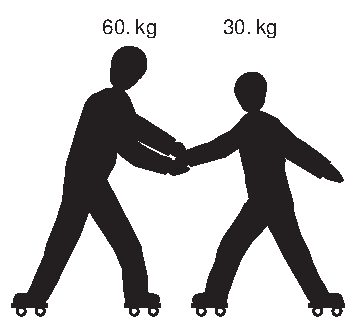
\includegraphics[keepaspectratio,scale=0.80]{Jan2005-Q04}
    \end{center}
    What is the magnitude of the impulse applied to the \SI{30}{\kilo\gram} roller-skater?
    \begin{multicols}{2}
    \begin{choices}
      \correctchoice{\SI{2.0}{\newton\second}}
        \wrongchoice{\SI{50}{\newton\second}}
        \wrongchoice{\SI{6.0}{\newton\second}}
        \wrongchoice{\SI{12}{\newton\second}}
    \end{choices}
    \end{multicols}
\end{question}
}

\element{nysed}{
\begin{question}{Jan2005-Q08}
    A lab cart is loaded with different masses and moved at various velocities.
    Which diagram shows the cart-mass system with the greatest inertia?
    \begin{multicols}{2}
    \begin{choices}
        %% NOTE: TODO: draw tikz
        \wrongchoice{
            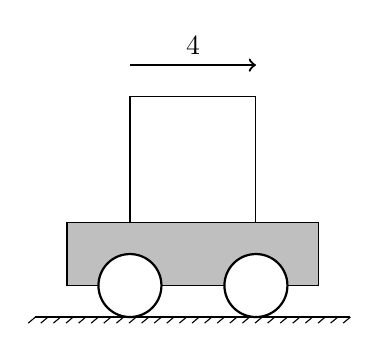
\begin{tikzpicture}[scale=0.80]
                %% Cart
                \draw[fill=black!25!white] (-2,0.5) rectangle (2,1.5);
                \draw[thick,fill=white] (-1.0,0.5) circle (0.5cm);
                \draw[thick,fill=white] (+1.0,0.5) circle (0.5cm);
                %% Mass
                \draw (-1.0,1.5) rectangle (1,3.5);
                \draw[thick,->] (-1,4) -- (1,4)
                    node[pos=0.5,anchor=south] {\SI{4}{\meter\per\second}};
                %% Ground
                \draw[thick] (-2.5,0) -- (2.5,0);
                \foreach \x in {-25,-23,...,25}
                    \draw[thin] (\x mm,0cm) -- ++ (220:0.15cm);
                %\node[anchor=north] at (0,-0.15) {Frictionless surface};
            \end{tikzpicture}
        }
        %\wrongchoice{\includegraphics[keepaspectratio,scale=0.66]{June2005-Q08-A}}
        %\wrongchoice{\includegraphics[keepaspectratio,scale=0.66]{June2005-Q08-B}}
        %\wrongchoice{\includegraphics[keepaspectratio,scale=0.66]{June2005-Q08-C}}
        %\correctchoice{\includegraphics[keepaspectratio,scale=0.66]{June2005-Q08-D}}
    \end{choices}
    \end{multicols}
\end{question}
}


%% Section June2004
%%--------------------
\element{nysed}{
\begin{question}{June2004-Q09}
    A \SI{50}{\kilo\gram} student threw a \SI{0.40}{\kilo\gram} ball with a speed of \SI{20}{\meter\per\second}.
    What was the magnitude of the impulse that the student exerted on the ball?
    \begin{multicols}{2}
    \begin{choices}
      \correctchoice{\SI{8.0}{\newton\second}}
        \wrongchoice{\SI{78}{\newton\second}}
        \wrongchoice{\SI{4.0e2}{\newton\second}}
        \wrongchoice{\SI{1.0e3}{\newton\second}}
    \end{choices}
    \end{multicols}
\end{question}
}

%% Section Jan2004
%%--------------------
\element{nysed}{
\begin{question}{Jan2004-Q05}
    Which object has the most inertia?
    \begin{choices}
        \wrongchoice{a \SI{0.001}{\kilo\gram} bumblebee traveling at \SI{2}{\meter\per\second}}
        \wrongchoice{a \SI{0.1}{\kilo\gram} baseball traveling at \SI{20}{\meter\per\second}}
        \wrongchoice{a \SI{5}{\kilo\gram} bowling ball traveling at \SI{3}{\meter\per\second}}
      \correctchoice{a \SI{10}{\kilo\gram} sled at rest}
    \end{choices}
\end{question}
}

\element{nysed}{
\begin{question}{Jan2004-Q12}
    What is the speed of a \SI{1.0e3}{\kilo\gram} car that has a momentum of \SI{2.0e4}{\kilo\gram\meter\per\second} east?
    \begin{multicols}{2}
    \begin{choices}
      \correctchoice{\SI{2.0e1}{\meter\per\second}}
        \wrongchoice{\SI{5.0e-2}{\meter\per\second}}
        \wrongchoice{\SI{1.0e4}{\meter\per\second}}
        \wrongchoice{\SI{2.0e7}{\meter\per\second}}
    \end{choices}
    \end{multicols}
\end{question}
}


%% Section June2003
%%--------------------
\element{nysed}{
\begin{question}{June2003-Q12}
    Ball $A$ of mass \SI{5.0}{\kilo\gram} moving at \SI{20}{\meter\per\second} collides with ball $B$ of unknown mass moving at \SI{10}{\meter\per\second} in the same direction.
    After the collision,
        ball $A$ moves at \SI{10}{\meter\per\second} and ball $B$ at \SI{15}{\meter\per\second},
        both still in the same direction.
    What is the mass of ball $B$?
    \begin{multicols}{2}
    \begin{choices}
      \correctchoice{\SI{10.}{\kilo\gram}}
        \wrongchoice{\SI{6.0}{\kilo\gram}}
        \wrongchoice{\SI{12.}{\kilo\gram}}
        \wrongchoice{\SI{2.0}{\kilo\gram}}
    \end{choices}
    \end{multicols}
\end{question}
}

\element{nysed}{
\begin{question}{June2003-Q15}
    Which person has the greatest inertia?
    \begin{choices}
      \correctchoice{a \SI{110}{\kilo\gram} wrestler resting on a mat}
        \wrongchoice{a \SI{90}{\kilo\gram} man walking at \SI{2}{\meter\per\second}}
        \wrongchoice{a \SI{70}{\kilo\gram} long-distance runner traveling at \SI{5}{\meter\per\second}}
        \wrongchoice{a \SI{50}{\kilo\gram} girl sprinting at \SI{10}{\meter\per\second}}
    \end{choices}
\end{question}
}

%% Section Aug2002
%%--------------------
\element{nysed}{
\begin{question}{Aug2002-Q25}
    Which is an acceptable unit for impulse?
    \begin{choices}
        \wrongchoice{newton meter (\si{\newton\meter})}
        \wrongchoice{joule per second (\si{\joule\per\second})}
        \wrongchoice{joule second (\si{\joule\second})}
      \correctchoice{kilogram meter per second (\si{\kilo\gram\meter\second})}
    \end{choices}
\end{question}
}

\element{nysed}{
\begin{question}{Aug2002-Q36}
    The diagram below shows a \SI{4.0}{\kilo\gram} cart moving to the right and a \SI{6.0}{\kilo\gram} cart moving to the left on a horizontal frictionless surface.
    \begin{center}
    \begin{tikzpicture}
        %% Ground
        \node[anchor=north,fill,pattern=north east lines,minimum width=8cm, minimum height=0.05cm] at (0,0) {};
        \draw (-4,0) -- (4,0);
        %% left Cart
        \node[draw,minimum height=1.0cm,minimum width=1.5cm,anchor=south] (L) at (-2.5,0.2) {\SI{4.0}{\kilo\gram}};
        \draw[fill=white] (L.south west) ++(0:0.4) circle (0.2);
        \draw[fill=black] (L.south west) ++(0:0.4) circle (1pt);
        \draw[fill=white] (L.south east) ++(180:0.4) circle (0.2);
        \draw[fill=black] (L.south east) ++(180:0.4) circle (1pt);
        \draw[thick,->] (L.north west) ++(90:0.5) -- ++(0:1.5) node[pos=0.5,anchor=south] {\SI{3.0}{\meter\per\second}};
        %% right Cart
        \node[draw,minimum height=1.2cm,minimum width=1.8cm,anchor=south] (R) at (+2.5,0.2) {\SI{6.0}{\kilo\gram}};
        \draw[fill=white] (R.south west) ++(0:0.3) circle (0.2);
        \draw[fill=black] (R.south west) ++(0:0.3) circle (1pt);
        \draw[fill=white] (R.south east) ++(180:0.3) circle (0.2);
        \draw[fill=black] (R.south east) ++(180:0.3) circle (1pt);
        \draw[thick,->] (R.north east) ++(90:0.5) -- ++(180:1.5) node[pos=0.5,anchor=south] {\SI{3.0}{\meter\per\second}};
    \end{tikzpicture}
    \end{center}
    When the two carts collide they lock together.
    The magnitude of the total momentum of the two-cart system after the collision is:
    \begin{multicols}{2}
    \begin{choices}
        \wrongchoice{\SI{0.0}{\kilo\gram\meter\per\second}}
      \correctchoice{\SI{6.0}{\kilo\gram\meter\per\second}}
        \wrongchoice{\SI{15}{\kilo\gram\meter\per\second}}
        \wrongchoice{\SI{30}{\kilo\gram\meter\per\second}}
    \end{choices}
    \end{multicols}
\end{question}
}


%% Section June2002
%%--------------------
\element{nysed}{
\begin{question}{June2002-Q11}
    A \SI{0.10}{\kilo\gram} model rocket's engine is designed to deliver an impulse of \SI{6.0}{\newton\second}.
    If the rocket engine burns for \SI{0.75}{\second},
        what average force does it produce?
    \begin{multicols}{2}
    \begin{choices}
        \wrongchoice{\SI{4.5}{\newton}}
      \correctchoice{\SI{8.0}{\newton}}
        \wrongchoice{\SI{45}{\newton}}
        \wrongchoice{\SI{80}{\newton}}
    \end{choices}
    \end{multicols}
\end{question}
}


%% Section Jan2002
%%--------------------
\element{nysed}{
\begin{question}{Jan2002-Q14}
    A bullet traveling at \SI{5.0e2}{\meter\per\second} is brought to rest by an impulse of \SI{50}{\newton\second}.
    What is the mass of the bullet?
    \begin{multicols}{2}
    \begin{choices}
        \wrongchoice{\SI{1.0e-2}{\kilo\gram}}
      \correctchoice{\SI{1.0e-1}{\kilo\gram}}
        \wrongchoice{\SI{1.0e1}{\kilo\gram}}
        \wrongchoice{\SI{2.5e4}{\kilo\gram}}
    \end{choices}
    \end{multicols}
\end{question}
}

%% NOTE: This might be cool to ask what the spring constant is
%% given the amount of compression, or give two values and state the difference
\element{nysed}{
\begin{question}{Jan2002-Q17}
    The diagram below shows two carts that were initially at rest on a horizontal,
        frictionless surface being pushed apart when a compressed spring attached to one of the carts is released.
    Cart $A$ has a mass of \SI{3.0}{\kilo\gram} and cart $B$ has a mass of \SI{5.0}{\kilo\gram}.
    \begin{center}
    \begin{tikzpicture}
        %% Ground
        \node[anchor=north,fill,pattern=north east lines,minimum width=8cm, minimum height=0.05cm] at (0,0) {};
        \draw (-4,0) -- (4,0);
        %% left Cart
        \node[draw,minimum height=1.0cm,minimum width=1.5cm,anchor=south] (L) at (-1.5,0.2) {\SI{3.0}{\kilo\gram}};
        \node[anchor=south] at (L.north) {$A$};
        \draw[fill=white] (L.south west) ++(0:0.4) circle (0.2);
        \draw[fill=black] (L.south west) ++(0:0.4) circle (1pt);
        \draw[fill=white] (L.south east) ++(180:0.4) circle (0.2);
        \draw[fill=black] (L.south east) ++(180:0.4) circle (1pt);
        \draw[thick,->] (L.west) -- ++(180:1.5) node[pos=0.5,anchor=south] {\SI{0.33}{\meter\per\second}};
        %% right Cart
        \node[draw,minimum height=1.3cm,minimum width=1.95cm,anchor=south] (R) at (+1.5,0.2) {\SI{5.0}{\kilo\gram}};
        \node[anchor=south] at (R.north) {$B$};
        \draw[fill=white] (R.south west) ++(0:0.3) circle (0.2);
        \draw[fill=black] (R.south west) ++(0:0.3) circle (1pt);
        \draw[fill=white] (R.south east) ++(180:0.3) circle (0.2);
        \draw[fill=black] (R.south east) ++(180:0.3) circle (1pt);
        \draw[thick,->] (R.east) -- ++(0:1.5);
        \draw[decoration={aspect=0.2,segment length=1.5mm,amplitude=3mm,coil},decorate] (R.west) -- ++(180:1);
    \end{tikzpicture}
    \end{center}
    If the speed of cart $A$ is \SI{0.33}{\meter\per\second} after the spring is released,
        what is the approximate speed of cart $B$ after the spring is released?
    \begin{multicols}{2}
    \begin{choices}
        \wrongchoice{\SI{0.12}{\meter\per\second}}
        \wrongchoice{\SI{0.33}{\meter\per\second}}
      \correctchoice{\SI{0.20}{\meter\per\second}}
        \wrongchoice{\SI{0.55}{\meter\per\second}}
    \end{choices}
    \end{multicols}
\end{question}
}


%% Section June2001
%%--------------------
\element{nysed}{
\begin{question}{June2001-Q13}
    The magnitude of the momentum of an object is \SI{64.0}{\kilo\gram\meter\per\second}.
    If the velocity of the object is doubled,
        the magnitude of the momentum of the object will be:
    \begin{multicols}{2}
    \begin{choices}
        \wrongchoice{\SI{32.0}{\kilo\gram\meter\per\second}}
        \wrongchoice{\SI{64.0}{\kilo\gram\meter\per\second}}
      \correctchoice{\SI{128}{\kilo\gram\meter\per\second}}
        \wrongchoice{\SI{256}{\kilo\gram\meter\per\second}}
    \end{choices}
    \end{multicols}
\end{question}
}

\element{nysed}{
\begin{question}{June2001-Q15}
    Satellite $A$ has a mass of \SI{1.5e3}{\kilo\gram} and is traveling east at \SI{8.0e3}{\meter\per\second}.
    Satellite $B$ is traveling west at \SI{6.0e3}{\meter\per\second}.
    The satellites collide head-on and come to rest.
    What is the mass of satellite $B$?
    \begin{multicols}{2}
    \begin{choices}
        \wrongchoice{\SI{2.7e3}{\kilo\gram}}
      \correctchoice{\SI{2.0e3}{\kilo\gram}}
        \wrongchoice{\SI{1.5e3}{\kilo\gram}}
        \wrongchoice{\SI{1.1e3}{\kilo\gram}}
    \end{choices}
    \end{multicols}
\end{question}
}


%% Section Jan2001
%%--------------------
\element{nysed}{
\begin{question}{Jan2001-Q11}
    Two cars having different weights are traveling on a level surface at difference constant velocities.
    Within the same time interval,
        greater force will always be required to stop the car that has the greater
    \begin{multicols}{2}
    \begin{choices}
        \wrongchoice{weight}
        \wrongchoice{kinetic energy}
        \wrongchoice{velocity}
      \correctchoice{momentum}
    \end{choices}
    \end{multicols}
\end{question}
}

\element{nysed}{
\begin{question}{Jan2001-Q12}
    A \SI{0.050}{\kilo\gram} bullet is fired from a \SI{4.0}{\kilo\gram} rifle that is initially at rest.
    If the bullet leaves the rifle with momentum having a magnitude of \SI{20}{\kilo\gram\meter\per\second},
        the rifle will recoil with a momentum having a magnitude of:
    \begin{multicols}{2}
    \begin{choices}
        \wrongchoice{\SI{1600}{\kilo\gram\meter\per\second}}
        \wrongchoice{\SI{80}{\kilo\gram\meter\per\second}}
      \correctchoice{\SI{20}{\kilo\gram\meter\per\second}}
        \wrongchoice{\SI{0.25}{\kilo\gram\meter\per\second}}
    \end{choices}
    \end{multicols}
\end{question}
}


%% Section June2000
%%--------------------
\element{nysed}{
\begin{question}{June2000-Q11}
    Compared to \SI{8}{\kilo\gram} of feathers,
        \SI{6}{\kilo\gram} grams of lead has:
    \begin{choices}
      \correctchoice{less mass and less inertia.}
        \wrongchoice{less mass and more inertia.}
        \wrongchoice{more mass and less inertia.}
        \wrongchoice{more mass and more inertia.}
    \end{choices}
\end{question}
}

\element{nysed}{
\begin{question}{June2000-Q15}
    A \SI{2.0}{\kilo\gram} cart moving due east at \SI{6.0}{\meter\per\second} collides with a \SI{3.0}{\kilo\gram} cart moving due west.
    The carts stick together and come to rest after the collision.
    What was the initial speed of the \SI{3.0}{\kilo\gram} cart?
    \begin{multicols}{2}
    \begin{choices}
        \wrongchoice{\SI{1.0}{\meter\per\second}}
        \wrongchoice{\SI{6.0}{\meter\per\second}}
        \wrongchoice{\SI{9.0}{\meter\per\second}}
      \correctchoice{\SI{4.0}{\meter\per\second}}
    \end{choices}
    \end{multicols}
\end{question}
}

\element{nysed}{
\begin{question}{June2000-Q16}
    What is the momentum of a \SI{1 200}{\kilo\gram} car traveling at \SI{15}{\meter\per\second} due east?
    \begin{choices}
        \wrongchoice{\SI{80}{\kilo\gram\meter\per\second} due east}
        \wrongchoice{\SI{80}{\kilo\gram\meter\per\second} due west}
      \correctchoice{\SI{1.8e4}{\kilo\gram\meter\per\second} due east}
        \wrongchoice{\SI{1.8e4}{\kilo\gram\meter\per\second} due west}
    \end{choices}
\end{question}
}


%% Section June1999
%%--------------------
\element{nysed}{
\begin{question}{June1999-Q12}
    What is the momentum of a \SI{1.5e3}{\kilo\gram} car as it travels at \SI{30}{\meter\per\second} due east for \SI{60}{\second}?
    \begin{choices}
      \correctchoice{\SI{4.5e4}{\kilo\gram\meter\per\second} east}
        \wrongchoice{\SI{4.5e4}{\kilo\gram\meter\per\second} west}
        \wrongchoice{\SI{2.7e6}{\kilo\gram\meter} east}
        \wrongchoice{\SI{2.7e6}{\kilo\gram\meter} west}
    \end{choices}
\end{question}
}

\element{nysed}{
\begin{question}{June1999-Q14}
    A \SI{2.0e3}{\kilo\gram} car collides with a tree and is brought to rest in \SI{0.50}{\second} by an average force of \SI{6.0e4}{\newton}.
    What is the magnitude of the impulse on the car during this \SI{0.50}{\second} interval?
    \begin{multicols}{2}
    \begin{choices}
        \wrongchoice{\SI{1.0e3}{\kilo\gram\second}}
      \correctchoice{\SI{3.0e4}{\newton\second}}
        \wrongchoice{\SI{1.2e5}{\newton\per\second}}
        \wrongchoice{\SI{6.0e7}{\newton\kilo\gram\second}}
    \end{choices}
    \end{multicols}
\end{question}
}

\element{nysed}{
\begin{question}{June1998-Q15}
    The velocity-time graph below represents the motion of a \SI{3}{\kilo\gram} cart along a straight line.
    The cart starts at $t=0$ and initially moves north.
    \begin{center}
    \begin{tikzpicture}
        \begin{axis}[
            axis y line=left,
            axis x line=middle,
            axis line style={->},
            ylabel={velocity},
            y unit=\si{\meter\per\second},
            ytick={-20,-10,0,10,20},
            xlabel={time},
            x unit=\si{\second},
            xtick={0,1,2,3,4,5,6,7},
            xmin=0,xmax=7.4,
            ymin=-22,ymax=22,
            grid=major,
            width=0.8\columnwidth,
            height=0.5\columnwidth,
            very thin,
        ]
        \addplot[line width=1pt,mark=\empty] plot coordinates {(0,0) (3,20) (7,-20)};
        \end{axis}
    \end{tikzpicture}
    \end{center}
    What is the magnitude of the change in momentum of the cart between $t=0$ and $t=3$ seconds?
    \begin{multicols}{2}
    \begin{choices}
        \wrongchoice{\SI{20}{\kilo\gram\meter\per\second}}
        \wrongchoice{\SI{30}{\kilo\gram\meter\per\second}}
      \correctchoice{\SI{60}{\kilo\gram\meter\per\second}}
        \wrongchoice{\SI{80}{\kilo\gram\meter\per\second}}
    \end{choices}
    \end{multicols}
\end{question}
}

\element{nysed}{
\begin{question}{June1999-Q18}
    In the diagram below, a \SI{100}{\kilo\gram} clown is fired from a \SI{500}{\kilo\gram} cannon.
    \begin{center}
        %% NOTE: too complex to bother
        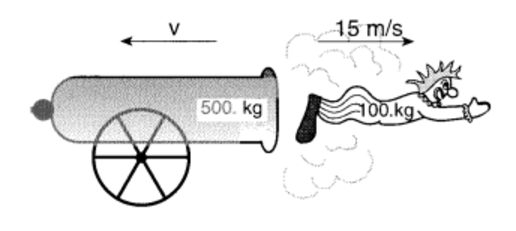
\includegraphics[keepaspectratio,scale=0.8]{June1999-Q18}
    \end{center}
    If the clown's speed is \SI{15}{\meter\per\second} after the firing,
        then the recoil speed ($v$) of the cannon is:
    \begin{multicols}{2}
    \begin{choices}
        \wrongchoice{\SI{75}{\meter\per\second}}
        \wrongchoice{\SI{15}{\meter\per\second}}
      \correctchoice{\SI{3.0}{\meter\per\second}}
        \wrongchoice{\SI{0}{\meter\per\second}}
    \end{choices}
    \end{multicols}
\end{question}
}


%% Section June1998
%%--------------------
\element{nysed}{
\begin{question}{June1998-Q51}
    During a collision between a photon and an electron,
        there is conservation of:
    \begin{choices}
        \wrongchoice{energy, only}
        \wrongchoice{momentum, only}
      \correctchoice{both energy and momentum}
        \wrongchoice{neither energy nor momentum}
    \end{choices}
\end{question}
}

\element{nysed}{
\begin{question}{June1998-Q54}
    As shown in the diagram below,
        a lump of clay travels horizontally to the right toward a block at rest on a frictionless surface.
    Upon collision, the clay and the block stick together and move to the right.
    \begin{center}
    \begin{tikzpicture}
        \begin{scope}[xshift=-2cm]
            %% Ground
            \node[anchor=north,fill,pattern=north east lines,minimum width=3.5cm, minimum height=0.05cm] at (0.25,0) {};
            \draw (-1.5,0) -- (2,0);
            %% block
            \node[draw,anchor=south,minimum size=0.75cm] (A) at (0.75,0) {};
            \node[anchor=south] at (A.north) {Block};
            %% clay
            \node[draw,circle,fill=white!60!black,minimum size=0.50cm] (B) at (-1,0.5) {};
            \node[anchor=south] at (B.north) {Clay};
            \draw[thick,->] (B.east) -- ++(0:0.5cm);
            %% label
            \node[anchor=north,yshift=-1em] at (0.25,0) {Before Collision};
        \end{scope}
        \begin{scope}[xshift=+2cm]
            %% Ground
            \node[anchor=north,fill,pattern=north east lines,minimum width=3.5cm, minimum height=0.05cm] at (0.25,0) {};
            \draw (-1.5,0) -- (2,0);
            %% clay
            \node[draw,circle,fill=white!60!black,minimum size=0.50cm] (B) at (0.5,0.5) {};
            \node[anchor=south east] at (B.north west) {Clay};
            %% block
            \node[draw,anchor=south,fill=white,minimum size=0.75cm] (A) at (1,0) {};
            \node[anchor=south] at (A.north) {Block};
            \draw[thick,->] (A.east) -- ++(0:0.5cm);
            %% label
            \node[anchor=north,yshift=-1em] at (0.25,0) {After Collision};
        \end{scope}
    \end{tikzpicture}
    \end{center}
    Compared to the total momentum of the clay and the block before the collision,
        the momentum of the clay-block system after the collisions is:
    \begin{multicols}{3}
    \begin{choices}
        \wrongchoice{less}
        \wrongchoice{greater}
      \correctchoice{the same}
    \end{choices}
    \end{multicols}
\end{question}
}


%% Section June1997
%%--------------------
\element{nysed}{
\begin{question}{June1997-Q10}
    A \SI{1000}{\kilo\gram} car traveling with a velocity of \SI[retain-explicit-plus]{+20}{\meter\per\second} decelerates at \SI{-5.0}{\meter\per\second\squared} until it comes to rest.
    What is the magnitude of the impulse applied to the car to bring it to rest?
    \begin{multicols}{2}
    \begin{choices}
        %% NOTE: kilogram meter per second?
        \wrongchoice{\SI{1.0e4}{\newton\second}}
      \correctchoice{\SI{2.0e4}{\newton\second}}
        \wrongchoice{\SI{3.9e4}{\newton\second}}
        \wrongchoice{\SI{4.3e4}{\newton\second}}
    \end{choices}
    \end{multicols}
\end{question}
}

%% NOTE: June1997-Q14 is dup of Jan2002-Q17

\element{nysed}{
\begin{question}{June1997-Q55}
    A student drops two eggs of equal mass simultaneously from the same height.
    Egg $A$ lands on the tile floor and breaks.
    Egg $B$ lands intact, without bouncing, on a foam pad lying on the floor.
    Compared to the magnitude of the impulse on egg $A$ as it lands, the magnitude of the impulse on egg $B$ as it lands is:
    \begin{multicols}{3}
    \begin{choices}
        \wrongchoice{less}
        \wrongchoice{greater}
      \correctchoice{the same}
    \end{choices}
    \end{multicols}
\end{question}
}


%% Section June1996
%%--------------------
\element{nysed}{
\begin{question}{June1996-Q17}
    A bullet traveling at \SI{5.0e2}{\meter\per\second} is brought to rest by an impulse of \SI{50}{\newton}.
    What is the mass of the bullet?
    \begin{multicols}{2}
    \begin{choices}
        \wrongchoice{\SI{2.5e4}{\kilo\gram}}
        \wrongchoice{\SI{1.0e1}{\kilo\gram}}
      \correctchoice{\SI{1.0e-1}{\kilo\gram}}
        \wrongchoice{\SI{1.0e-2}{\kilo\gram}}
    \end{choices}
    \end{multicols}
\end{question}
}

%% Section June1995
%%--------------------
\element{nysed}{
\begin{question}{June1995-Q13}
    If a net force of \SI{10}{\newton} acts on a \SI{6.0}{\kilo\gram} mass for \SI{8.0}{\second},
        the total change of momentum of the mass is:
    \begin{multicols}{2}
    \begin{choices}
        \wrongchoice{\SI{48}{\kilo\gram\meter\per\second}}
        \wrongchoice{\SI{60}{\kilo\gram\meter\per\second}}
      \correctchoice{\SI{80}{\kilo\gram\meter\per\second}}
        \wrongchoice{\SI{480}{\kilo\gram\meter\per\second}}
    \end{choices}
    \end{multicols}
\end{question}
}

\element{nysed}{
\begin{question}{June1995-Q14}
    In the diagram below, a \SI{0.4}{\kilo\gram} steel sphere and a \SI{0.1}{\kilo\gram} wooden sphere are located \SI{2.0}{\meter} above the ground.
    Both sphere are allowed to fall from rest.
    \begin{center}
    \begin{tikzpicture}
        %% ground
        \draw (-3,0) -- (3,0);
        \node[anchor=north,minimum width=6cm,pattern=north east lines] at (0,0) {};
        \node[anchor=north] at (0,-1em) {Ground};
        %% Labels
        \draw[dashed] (-3,2) -- (3,2);
        \draw[dashed] (-3,4) -- (3,4);
        \draw[latex-latex] (-2.5,0) -- (-2.5,4) node[pos=0.33,anchor=center,fill=white] {\SI{2.0}{\meter}};
        \draw[latex-latex] (-1.5,2) -- (-1.5,4) node[pos=0.5,anchor=center,fill=white] {\SI{1.0}{\meter}};
        %% Wood
        \draw[fill=black] (+2,4.15) circle (0.15cm) node[anchor=south,yshift=0.15cm] {Wood};
        %% Steel
        \draw[fill=white!90!black] (0,4.15) circle (0.15cm) node[anchor=south,yshift=0.15cm] {Steel};
    \end{tikzpicture}
    \end{center}
    Which statement best describes the spheres after they have fallen \SI{1.0}{\meter}?
    [Neglect air resistance.]
    \begin{choices}
        \wrongchoice{both spheres have the same speed and momentum}
      \correctchoice{both spheres have the same speed and the steel sphere has more momentum than the wooden sphere.}
        \wrongchoice{the steel sphere has greater speed and has less momentum than the wooden sphere.}
        \wrongchoice{the steel sphere has greater speed than the wooden sphere and both spheres have the same momentum.}
    \end{choices}
\end{question}
}


%% Section June1994
%%--------------------
\element{nysed}{
\begin{question}{June1994-Q15}
    A \SI{2.0}{\kilo\gram} toy cannon is at rest on a frictionless surface.
    A remote triggering device causes a \SI{0.005}{\kilo\gram} projectile to be fired from the cannon.
    Which equation describes this system after the cannon is fired?
    \begin{choices}
        \wrongchoice{mass of cannon + mass of projectile = 0}
        \wrongchoice{speed of cannon + speed of projectile = 0}
      \correctchoice{momentum of cannon + momentum of projectile = 0}
        \wrongchoice{velocity of cannon + velocity of projectile = 0}
    \end{choices}
\end{question}
}


%% Section June1990
%%--------------------
\element{nysed}{
\begin{question}{June1990-Q07}
    Which pair of terms are vector quantities?
    \begin{choices}
        \wrongchoice{force and mass}
        \wrongchoice{distance and displacement}
      \correctchoice{momentum and acceleration}
        \wrongchoice{speed and velocity}
    \end{choices}
\end{question}
}

\element{nysed}{
\begin{question}{June1990-Q11}
    A spring is compressed between two stationary blocks as shown in the diagram below.
    Block $A$ has mass of \SI{6.0}{\kilo\gram}.
    After the spring is released, block $A$ moves west at \SI{8.0}{\meter\per\second} and block $B$ moves east at \SI{16}{\meter\per\second}.
    \begin{center}
    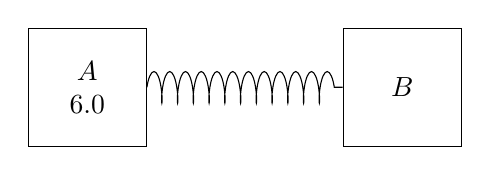
\begin{tikzpicture}
        %% block A and B
        \node[draw,minimum size=1.5cm,anchor=center,text centered,text width=2em] (A) at (-2,0) {$A$ \SI{6.0}{\kilo\gram}};
        \node[draw,minimum size=1.5cm,anchor=center,text centered,text width=2em] (B) at (+2,0) {$B$};
        %% spring
        \draw[decoration={aspect=0.2,segment length=2.0mm,amplitude=2mm,coil},decorate] (A.east) -- (B.west);
    \end{tikzpicture}
    \end{center}
    What is the mass of block $B$?
    [Assume no frictional effects.]
    \begin{multicols}{2}
    \begin{choices}
        \wrongchoice{\SI{16}{\kilo\gram}}
        \wrongchoice{\SI{12}{\kilo\gram}}
      \correctchoice{\SI{3.0}{\kilo\gram}}
        \wrongchoice{\SI{6.0}{\kilo\gram}}
    \end{choices}
    \end{multicols}
\end{question}
}

\element{nysed}{
\begin{question}{June1990-Q14}
    A \SI{25}{\kilo\gram} mass travels east with a constant velocity of \SI{40}{\meter\per\second}.
    The momentum of this mass is:
    \begin{multicols}{2}
    \begin{choices}
      \correctchoice{\SI{1.0e3}{\kilo\gram\meter\per\second} east}
        \wrongchoice{\SI{9.8e3}{\kilo\gram\meter\per\second} east}
        \wrongchoice{\SI{1.0e3}{\kilo\gram\meter\per\second} west}
        \wrongchoice{\SI{9.8e3}{\kilo\gram\meter\per\second} west}
    \end{choices}
    \end{multicols}
\end{question}
}

\element{nysed}{
\begin{question}{June1990-Q16}
    A constant braking force of \SI{10}{\newton} applied for \SI{5}{\second} is used to stop a \SI{2.5}{\kilo\gram} cart traveling at \SI{20}{\meter\per\second}.
    The magnitude of the impulse applied to stop the cart is:
    \begin{multicols}{2}
    \begin{choices}
        \wrongchoice{\SI{10}{\newton\second}}
        \wrongchoice{\SI{30}{\newton\second}}
      \correctchoice{\SI{50}{\newton\second}}
        \wrongchoice{\SI{100}{\newton\second}}
    \end{choices}
    \end{multicols}
\end{question}
}


%% Section June1989
%%--------------------
\element{nysed}{
\begin{question}{June1989-Q17}
    What is the magnitude of the velocity of a \SI{25}{\kilo\gram} mass that is moving with a momentum of \SI{100}{\kilo\gram\meter\per\second}?
    \begin{multicols}{2}
    \begin{choices}
        \wrongchoice{\SI{0.25}{\meter\per\second}}
        \wrongchoice{\SI{2500}{\meter\per\second}}
        \wrongchoice{\SI{40}{\meter\per\second}}
      \correctchoice{\SI{4.0}{\meter\per\second}}
    \end{choices}
    \end{multicols}
\end{question}
}


%% Section June1986
%%--------------------
\element{nysed}{
\begin{question}{June1986-Q10}
    If the direction of the momentum of an object is west,
        the direction of the velocity of the object is:
    \begin{multicols}{2}
    \begin{choices}
        \wrongchoice{north}
        \wrongchoice{south}
        \wrongchoice{east}
      \correctchoice{west}
    \end{choices}
    \end{multicols}
\end{question}
}

\element{nysed}{
\begin{question}{June1986-Q11}
    An impulse $I$ is applied to an object.
    The change in the momentum of the object is:
    \begin{multicols}{4}
    \begin{choices}
      \correctchoice{$I$}
        \wrongchoice{$2I$}
        \wrongchoice{$\dfrac{I}{2}$}
        \wrongchoice{$4I$}
    \end{choices}
    \end{multicols}
\end{question}
}

\element{nysed}{
\begin{question}{June1986-Q12}
    An \SI{80}{\kilo\gram} skater and a \SI{60}{\kilo\gram} skater stand at rest in the center of a skating rink.
    The two skaters push each other apart.
    The \SI{60}{\kilo\gram} skater moves with a velocity of \SI{10}{\meter\per\second} east.
    What is the velocity of the \SI{80}{\kilo\gram} skater?
    [Neglect any frictional effects.]
    \begin{multicols}{2}
    \begin{choices}
        \wrongchoice{\SI{0.13}{\meter\per\second} west}
      \correctchoice{\SI{7.5}{\meter\per\second} west}
        \wrongchoice{\SI{10}{\meter\per\second} east}
        \wrongchoice{\SI{13}{\meter\per\second} east}
    \end{choices}
    \end{multicols}
\end{question}
}





\endinput


